% !TeX root = ../main.tex

\chapter{基于双层缓存的优先经验回放算法}\label{chap:dper}

在第~\ref{chap:intro}~章中我们已经介绍,尽管使用随机抽取经验样本进行回放的做法能够对算法样本效率起到一定的优化,但是仍然较为局限。而PER算法在样本池中按优先级进行经验回放的做法则更加有效,能够给更重要的样本赋予更高的优先级,确保更有价值的经验得到更多的回放,从而起到了提升样本效率的效果。在PER算法中,理想的设计方案是计算样本池中的样本被用于学习的次数,次数越少,说明该样本越应被优先提供给智能体进行学习。考虑到该指标在实际运行时难以获取,选择了使用时序差分误差来辅助计算样本池中的采样优先级作为替代方案,这是因为时序差分误差大的样本,意味着策略在该样本所处状态上的决策效果存在较大改进空间,同样可以被认为是更有高学习价值的经验样本,因此需要为其分配更高的优先级进行学习。尽管优先经验回放方法已经在强化学习中取得了很好的效果,但它仍有很多局限性:

\begin{enumerate}
    \item 为避免扫描整个样本回放池的昂贵成本,只有被回放过的经验样本的时序差分误差值会被更新,这将导致一些有较小的初始误差值样本长时间不被回放,进而对整个样本空间覆盖率不高
    \item 时序差分误差对噪声非常敏感,很容易因噪声而增加估计误差,同时较高的时序差分误差带来的频繁回放会因损失多样性而导致算法过拟合
    \item PER只对由访问过的状态组成的回放样本池进行优先级分配。与整个状态空间相比,样本池可能只覆盖其中一个小的子集,实际中并不能实现全局意义上的优先级分配就无法实现,与其设计理念相差甚远。
\end{enumerate}

这些问题在现有的工作中并没有得到太多关注,为此,我们设计了基于双层缓存的优先经验回放算法,可以有效解决上述提到的优先经验回放算法的局限性,学习更多的重要经验,提升强化学习的样本效率效率。

\section{双层经验样本回放池及回放算法设计}

\begin{figure}[ht]
\centering
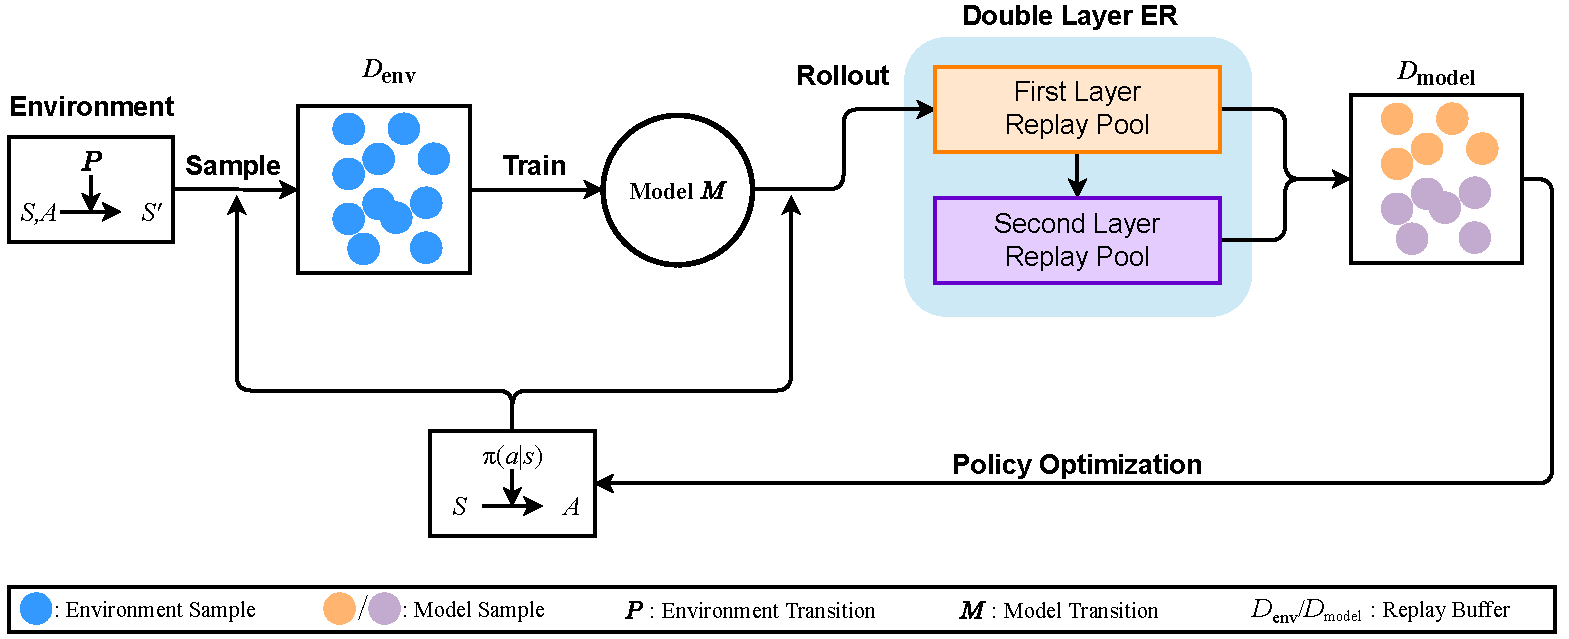
\includegraphics[width=\textwidth]{figures/dber.pdf}
\caption{基于双层缓存的优先经验回放算法示意图}
\label{fig:algo-structure}
\end{figure}

在优先经验回放算法的基础上,本文设计了一个双层经验回放池。在原有的单层样本池基础上增加了第二层回放缓冲区。与通常的经验重放方法一样,它首先将观察到的样本存储在第一层经验回放池中,当第一层样本池填充满后,随机抽取一定比例的样本填入第二层回放缓冲区中。在这样的设计下,第二层的样本累积速度将会比第一层大幅减缓,也意味着第二层回放池中将会缓存更长时间的历史经验,对整体样本空间起到更好的覆盖效果。这样设计的动机是,当人类在从经验中学习时,并不会一位的按照固定速度从历史经验中进行回放学习,而是更高频地对短期经验进行快速回放、更低频地对长期经验进行慢速回放,从而既能实时更新最新的知识,也能更充分利用上较长时间的经验。

在该样本池的设计下,我们对第一层和第二层的样本分别按照时序差分误差进行优先级排序,并将两层样本池中的样本取出进行混合回放学习,以实现不同速度的经验混合回放,从而生成更理想的优先经验回放样本分布。算法的结构示意图如图~\ref{fig:algo-structure}~所示。


\section{DPER算法描述与设计}

在本小节中,我们将介绍双层优先经验回放算法以及它如何帮助提高强化学习的样本效率。

首先使用策略与环境交互得到环境数据$\mathcal{D}_{\text{env}}$,并根据$\mathcal{D}_{\text{env}}$训练得到环境模型。得到模型后,我们先生成一定量的样本$(s_t, a_t, s_{t+1}, r_{t+1})$填充到第一层经验回放池中,并按照时序差分误差进行优先级排序。当第一层回放池填充完毕后,我们抽取一定比例的样本存入第二层缓存池中,并对其也进行一次时序差分误差优先级排序。随后将两层回放池中的样本进行混合回放提供给智能体进行策略优化学习。

策略优化更新后的策略将会重新与环境交互,生成新的交互样本用于改进环境模型的学习,而模型则会继续生成模拟数据填充加入双层样本回放池中。与基于模型的强化学习方法相结合,主要目的是为了能更快地生成样本,确保优先回放算法能更快地填充样本池并进行回放学习。

此外,为了能够让双层回放的设计更加灵活,我们设计了一个动态控制第二次回放池大小的机制,通过参数$\alpha\in[0,1]$控制第二层回放池容量大小。具体的做法是,我们在每次循环中抽取$\alpha$百分比的样本用于填充进第二层回放池,剩余$(1-\alpha)$百分比的样本则用于常规经验学习。参数$\alpha$的设定既可以是一个固定的值,也可以是一个随时间衰退的变量。

我们称上述所设计的算法为基于双层缓存的优先经验回放算法(Double-layer Prioritized Experience Replay,DPER)。流程的概述如算法~\ref{algo:dper-method}~所展示。

\begin{algorithm}[t]
\caption{基于双层缓存的优先经验回放算法}
\label{algo:dper-method}
\begin{algorithmic}
\STATE 初始化超参数 $\alpha$、策略 $\pi_\theta$、环境样本回放池 $\mathcal{D}_{\mathrm{env}}$、模型样本回放池 $\mathcal{D}_{\mathrm{model}}$\\
\FOR{$N_\mathrm{epoch}$ 迭代次数}
    \STATE 在环境中基于策略 $\pi_\theta$ 采取行动进行交互
    \STATE 将生成的交互样本填充至 $\mathcal{D}_{\mathrm{env}}$\\
    \FOR{$N_\mathrm{train}$ 迭代次数}
        \STATE 基于样本回放池 $\mathcal{D}_{\mathrm{env}}$训练概率模型$\mathcal{M}_\phi$\\
        \STATE 建立模型子集$\mathcal{M} = \{\mathcal{M}_{\phi_1},\ldots,\mathcal{M}_{\phi_{N}}\}$\\
        \FOR{$t=1,2,\ldots ,T$}
            \STATE 从模型子集$\mathcal{M}$中随机抽取一个模型$\mathcal{M}_{\phi_t}$\\
            \STATE 在模型 $\mathcal{M}_{\phi_t}$ 上使用策略 $\pi_\theta$ 生成模拟样本 $x=\left(s_{t+1},s_t,a_t\right)$ \\
            \STATE 将样本填入第一层样本回放池 $\mathcal{B}_1$中\\
        \ENDFOR
        \STATE 根据是时序差分误差计算 $\mathcal{B}_1$ 的优先级并排序\\
        \FOR{$x\in \mathcal{B}_1$}
            \IF{随机数 $p\sim U(0,1)\leq \alpha$}
                \STATE 将样本 $x$ 按排序后的顺序填充至第二层样本池 $\mathcal{B}_{2}$中
            \ENDIF
        \ENDFOR
        \STATE 将两层样本池进行临时拼接: $\mathcal{D}_{\mathrm{model}}\leftarrow\mathcal{D}_{\mathrm{model}}\bigcup(\mathcal{B}_2\bigoplus\mathcal{B}_1)$ ($\bigoplus$ 表示集合拼接)
    \ENDFOR
    \STATE 在 $\mathcal{D}_{\mathrm{model}}$上进行 $\pi_\theta$的优化: $\theta\leftarrow \theta - \lambda\nabla_\theta J_\theta(\mathcal{D}_{\mathrm{model}})$
\ENDFOR
\end{algorithmic}
\end{algorithm}

\section{实验设计与分析}

\subsection{Cliff-Walking环境实验设计与分析}

\begin{figure}[t]
\centering
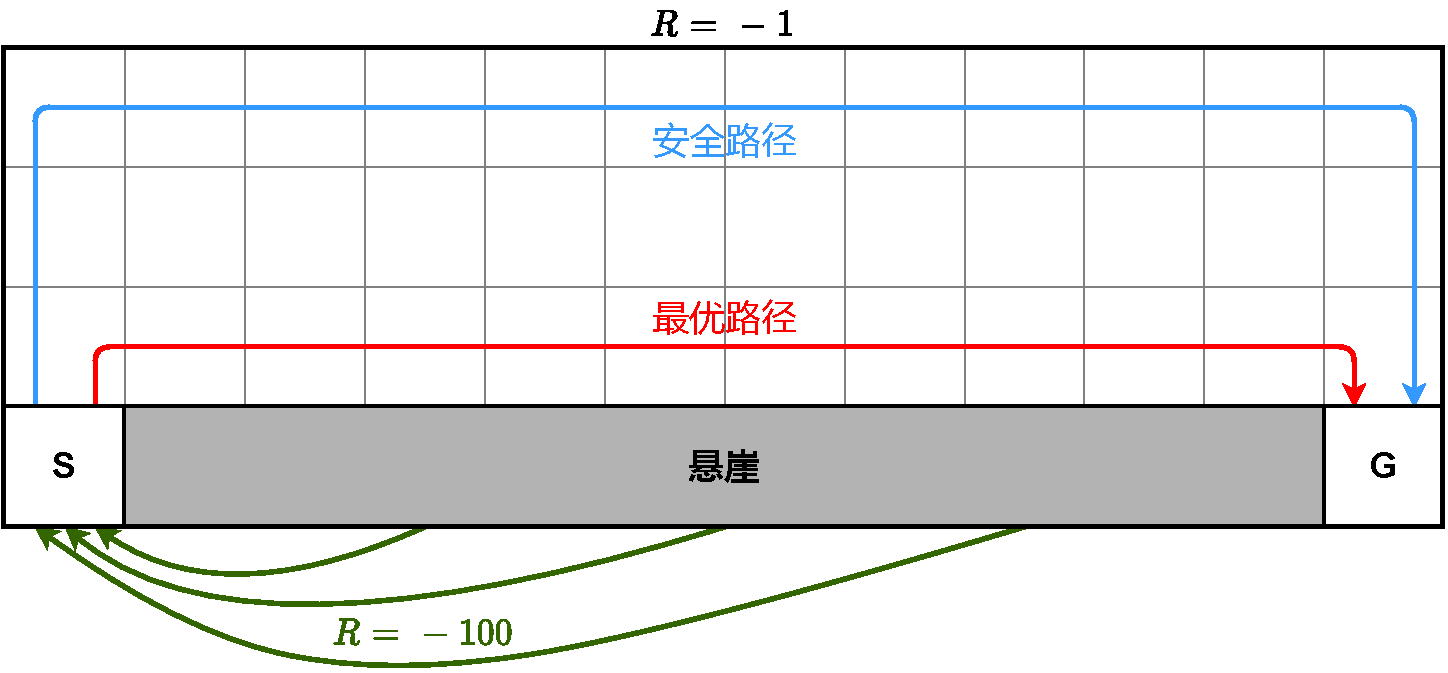
\includegraphics[width=\textwidth]{figures/cliff-env.pdf}
\caption{Cliff-Walking实验环境示意图}
\label{fig:cliff-env}
\end{figure}


为了直观理解双层经验重放的潜在好处,我们先设计了一组简单环境下的实验,引入了Cliff-Walking环境(如图~\ref{fig:cliff-env}~所示)。在该环境由$4\times 12$个方格组成,每次只能由一个方格移动到另一个相邻方格,并获得$R=-1$的反馈值,任务目标是从起始状态S出发,以尽可能快的速度到达终点状态G。如果智能体在行动过程中进入灰色的悬崖区域,则会直接返回初始状态S并得到$R=-100$的反馈值。显然,在Cliff-Walking环境下只存在唯一的最优路径,如图中的红线所示。然而,这条最优路径也是最危险的路径。如果算法在早期阶段效率不高,随时可能不小心从最优路径进入悬崖,造成较大的惩罚,从而影响算法的收敛性。在该环境下算法样本效率的提升会显著改善训练曲线的收敛速度。

我们使用优先经验算法(PER)作为基线进行测试,并设计了一个双层回放池的优先经验回放算法。表~\ref{tab:cliff-stats}~的实验结果显示了在Cliff-Walking环境下使用单层或双层重放缓冲区的PER算法统计结果。这些指标代表了智能体落入悬崖区的概率以及平均收益。每次实验的运行由3组随机种子生成,每次实验需要2000步。统计结果表明,用双层经验重放法训练的策略落入悬崖区的次数较少,在评估过程中表现出更好的稳健性。可以看出,当使用双层回放池时,PER算法的表现比单层回放缓冲器的整体表现要好。

\begin{table}[ht]
\centering
\begin{tabular}{l|l|l|l|l|l} 
\toprule
                                                    & Layer  & Seed 1           & Seed 2           & Seed 3           & Avg.              \\ 
\hline
\multirow{2}{*}{$P_\text{mean}(\text{Fail})$~ (\%)} & single & 0.645            & 0.678            & 0.611            & 0.645             \\ 
\cline{2-6}
                                                    & double & \textbf{0.357}   & \textbf{0.332}   & \textbf{0.312}   & \textbf{0.335}    \\ 
\hline
\multirow{2}{*}{$P_\text{std}(\text{Fail})$~ (\%)}  & single & 0.294            & 0.318            & 0.337            & 0.316             \\ 
\cline{2-6}
                                                    & double & \textbf{0.201}   & \textbf{0.197}   & \textbf{0.185}   & \textbf{0.194}    \\ 
\hline
\multirow{2}{*}{$R_\text{mean}$}                    & single & -13.258          & \textbf{-13.179} & -14.188          & -13.542           \\ 
\cline{2-6}
                                                    & double & \textbf{-12.978} & -13.205          & \textbf{-13.189} & \textbf{-13.124}  \\ 
\hline
\multirow{2}{*}{$R_\text{std}$}                     & single & 4.038            & 3.971            & 3.862            & 3.957             \\ 
\cline{2-6}
                                                    & double & \textbf{2.225}   & \textbf{2.378}   & \textbf{2.804}   & \textbf{2.469}    \\
\bottomrule
\end{tabular}
\caption{Result of Cliff Walking}
\label{tab:cliff-stats}
\end{table}

\begin{figure}[t]
\centering
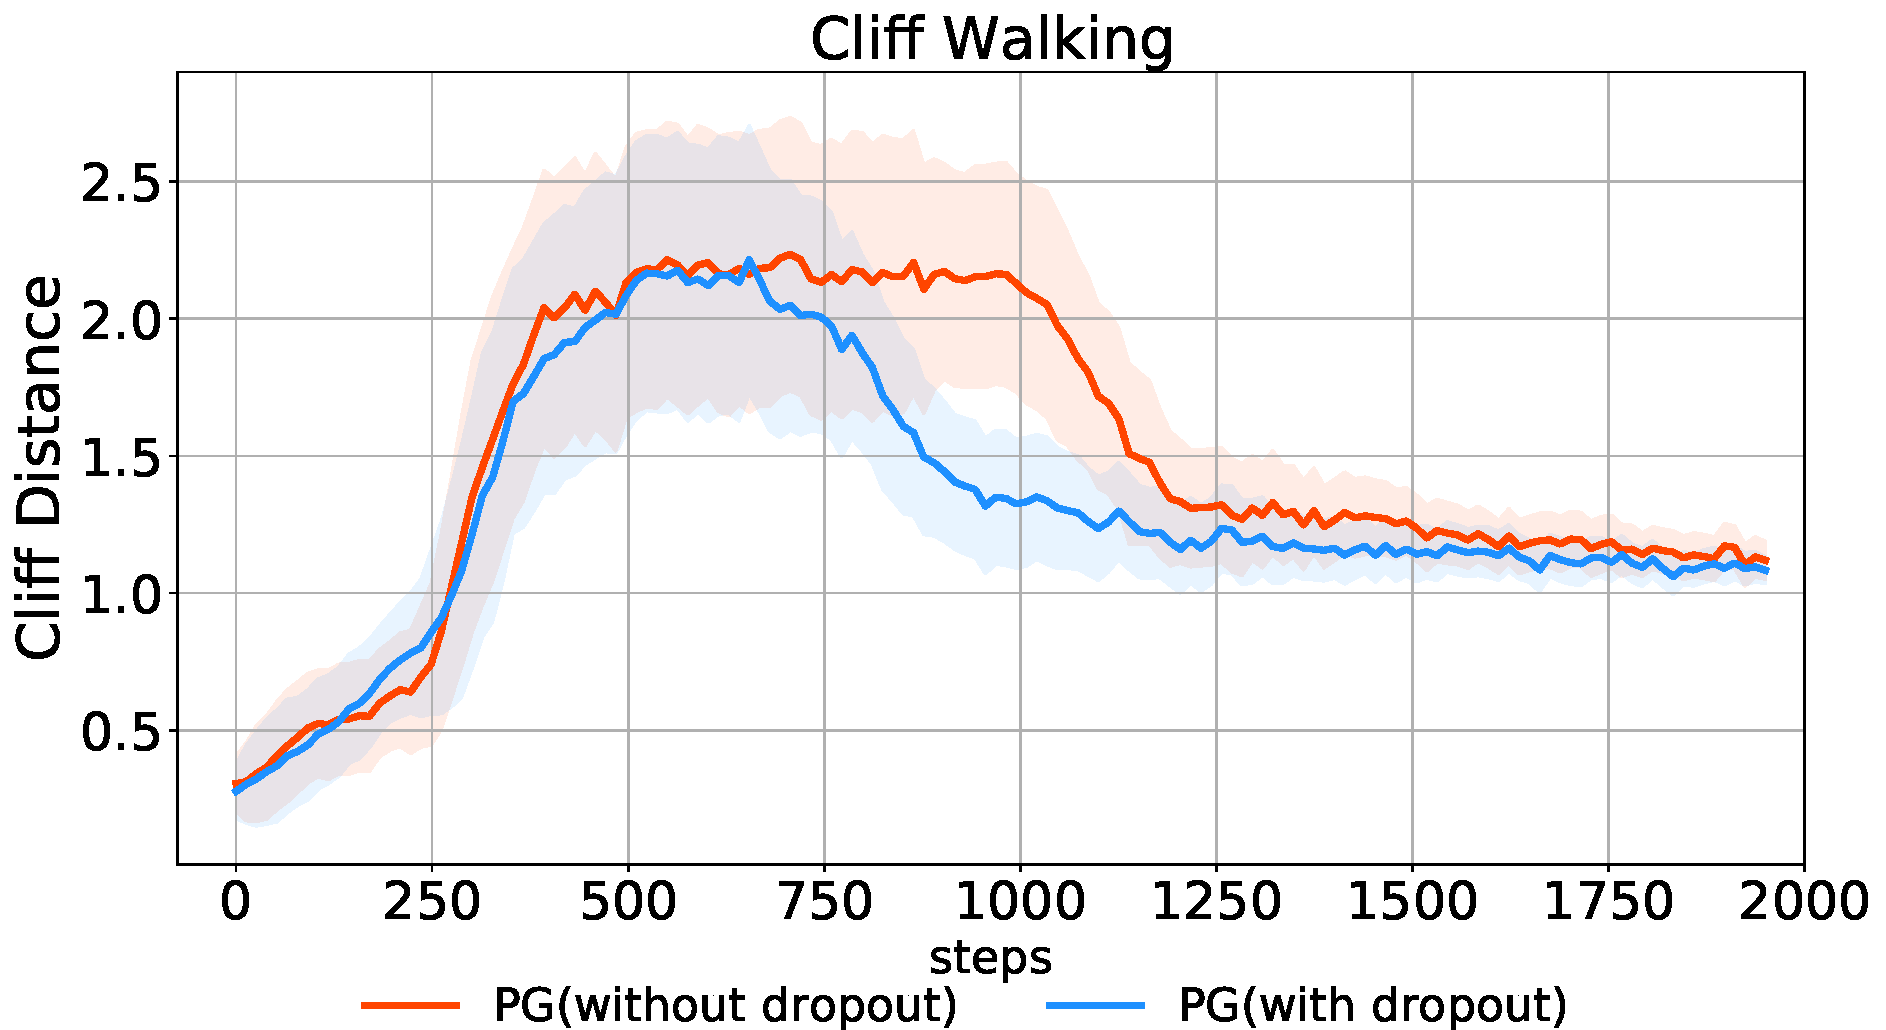
\includegraphics[width=\textwidth]{figures/cliffwalking.pdf}
\caption{Cliff-Walking实验结果曲线}
\label{fig:cliff-dis}
\end{figure}

图~\ref{fig:cliff-dis}~展示了使用单层优先经验回放(红线)和双层优先经验回放(蓝线)在Cliff-Walking环境上训练时智能体距离悬崖边缘的距离。如图中训练曲线所示,原始PER算法中的智能体倾向于从远离悬崖的安全路径进行探索,直到它获得足够的信息来慢慢接近最优路径。相比之下,具有双层经验回放的PER算法能够更快地学习,并且能够更有把握地提前接近危险区域,从而更好地收敛到最优路径。可以看出使用了双层经验回放的算法可以更快的选择接近悬崖的最优路径,说明了DPER算法能够有效地提升学习速度,增加样本利用效率。

\subsection{Mujoco环境实验设计与分析}

在本次验证实验中,我们选用了OpenAI-Gym库中的经典Mujoco仿真环境\cite{todorov2012mujoco}用于验证,具体地,我们选择了Mujoco下的Hopper,Walker,HalfCheetah和Ant这四个环境,他们都是验证智能体在连续动作条件下决策性能的常用测试环境,这四个环境的具体测试任务如下描述。

\begin{itemize}
    \item \textbf{Hopper}: 控制一个单腿机器人尽可能快地向前行走。
    \item \textbf{Walker2d}: 控制一个双腿机器人尽可能快地往前行走。
    \item \textbf{HalfCheetah}: 控制一个双腿爬行机器人尽可能快地向前行走。
    \item \textbf{Ant}: 控制一个四腿爬行机器人尽可能快地向前行走。
\end{itemize}

\begin{figure}[t]
    \centering
    \subcaptionbox{Hopper}{
        \centering
        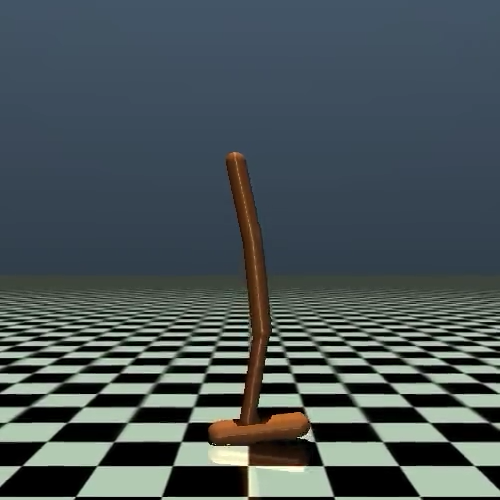
\includegraphics[width=0.48\textwidth]{figures/hopper.png}
        \label{fig:hopper}
    }
    \subcaptionbox{Walker}{
        \centering
        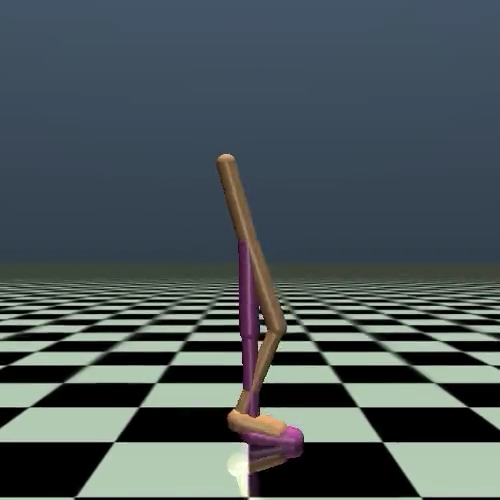
\includegraphics[width=0.48\textwidth]{figures/walker.png}
        \label{fig:walker}
    }
    \\
    \subcaptionbox{HalfCheetah}{
        \centering
        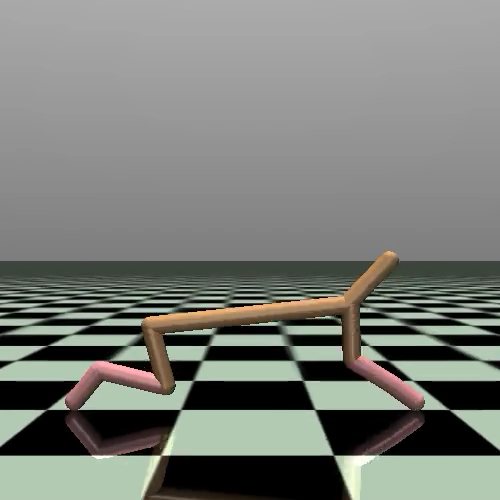
\includegraphics[width=0.48\textwidth]{figures/cheetah.png}
        \label{fig:cheetah}
    }
    \subcaptionbox{Ant}{
        \centering
        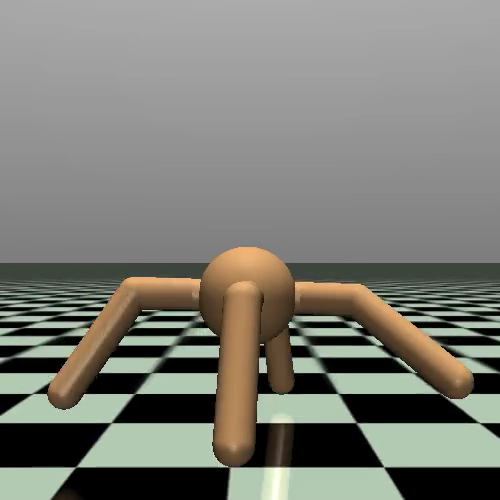
\includegraphics[width=0.48\textwidth]{figures/ant.png}
        \label{fig:ant}
    }
    \caption{实验所使用的四种仿真Mujoco环境示意图}
    \label{fig:env-figures}
\end{figure}

在本实验中,我们关于样本效率对比了多个基线方法,将基于模型的强化学习算法中的代表算法MBPO\cite{janner2019trust},以及它与PER \cite{schaul2016prioritized}的结合MBPO+PER进行了对比实验。在不同环境的实验中所使用的参数设定如表~\ref{tab:parameters}所示。

\begin{table}[htbp]
\centering
\begin{tabular}{c|c|c|c|c|c} 
\toprule
Env         & Epochs & $\alpha$ & \begin{tabular}[c]{@{}l@{}}buffer\\size\end{tabular} & \begin{tabular}[c]{@{}l@{}}env steps\\per epoch\end{tabular} & \begin{tabular}[c]{@{}l@{}}model steps\\per epoch\end{tabular}  \\ 
\hline
Hopper      & 120    & 0.2      & $10^5$                                              & 1000                                                         & 100                                                             \\ 
\hline
Walker      & 300    & 0.2      & $10^5$                                              & 1000                                                         & 100                                                             \\ 
\hline
HalfCheetah & 400    & 0.2      & $10^5$                                              & 1000                                                         & 200                                                             \\ 
\hline
Ant         & 300    & 0.2      & $10^5$                                              & 1000                                                         & 100                                                             \\
\bottomrule
\end{tabular}
\caption{Mujoco实验参数设定}
\label{tab:parameters}
\end{table}

具体而言,我们在Hopper环境运行了120轮循环,每轮循环包含1000步更新;相对应地,我们在Walker环境运行了300轮循环$\times$1000步;在HalfCheetah环境运行率400轮循环$\times$1000步;在Ant环境运行了300轮循环$\times$1000步。环境模型所使用的神经网络结构为$4\times 200$多层感知机(MLP)结构,这些模型在学习后均被用于预测未来100步的状态转移过程。

\begin{figure}[H]
  \centering
  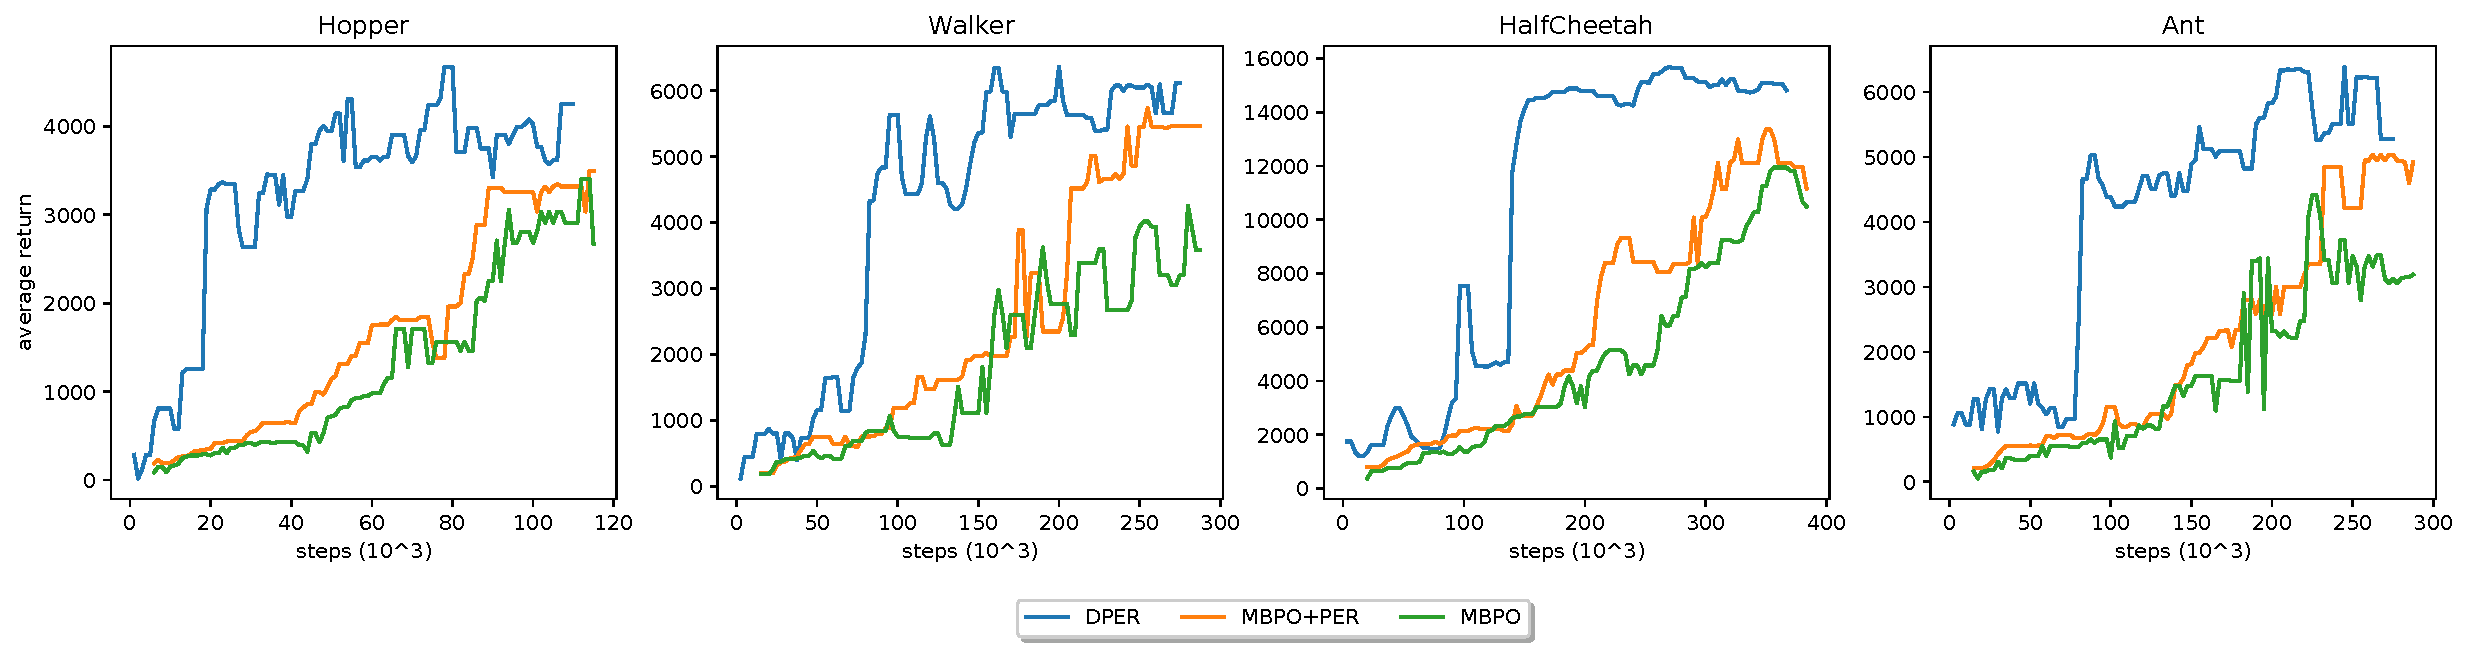
\includegraphics[width=\textwidth]{figures/dler.pdf}
  \caption{DPER算法与其他基线算法在不同环境下的训练曲线}
  \label{fig:dper-performance}
\end{figure}

在这些参数设定下,最终的训练曲线如图~\ref{fig:dper-performance}所示。可以看出,DPER算法由于双层缓存的优化,取得了远超其他算法的性能。

为了进一步确定DPER算法中参数$\alpha$的取值,我们还进行了一组参数实验,实验结果如表~\ref{tab:dper-ablation}所示。可以看出,当$\alpha$取值为0.2左右时将能取得最好的性能优化效果。

\begin{table}[ht]
\centering
\resizebox{\columnwidth}{!}{
\begin{tabular}{c|c|c|c|c|c|c} 
\toprule[2pt]
$\alpha$                           & 0       & 0.1     & 0.2             & 0.3              & 0.4     & 0.5      \\ 
\hline
$R_\text{avg}(\text{Hopper})$      & 3985.4  & 4057.1  & \textbf{4166.2} & 4030.7           & 3864.5  & 3796.5   \\ 
\hline
$R_\text{avg}(\text{Walker})$      & 5738.2  & 5943.4  & \textbf{6083.8} & 6008.1           & 5882.9  & 5694.4   \\ 
\hline
$R_\text{avg}(\text{HalfCheetah})$ & 15479.5 & 15630.1 & 15879.2         & \textbf{16036.1} & 15640.4 & 15038.1  \\ 
\hline
$R_\text{avg}(\text{Ant})$         & 5975.2  & 6023.5  & \textbf{6249.8} & 6199.5           & 6047.1  & 5926.3   \\
\bottomrule[2pt]
\end{tabular}
}
\caption{Result of Ablation Study}
\label{tab:dper-ablation}
\end{table}

\section{本章小结}

本章主要介绍了针对强化学习的样本利用效率问题所提出了基于双层缓存的优先经验回放算法(Double-layer Prioritized Experience Replay,DPER)。DPER算法通过双层经验回放池的设计,在添加的第二层经验回放池中以更慢的速率全局空间的经验样本进行回放缓存,提高了经验回放样本在整体样本空间中的有效覆盖率,加速了策略学习速度,最终实现了算法样本利用效率的提升。在CliffWalking和Mujoco中的Hopper、Walker2d、HalfCheetah、Ant仿真环境下均验证了DPER算法在样本利用效率的提升效果。